% Options for packages loaded elsewhere
\PassOptionsToPackage{unicode}{hyperref}
\PassOptionsToPackage{hyphens}{url}
%
\documentclass[
]{article}
\usepackage{amsmath,amssymb}
\usepackage{iftex}
\ifPDFTeX
  \usepackage[T1]{fontenc}
  \usepackage[utf8]{inputenc}
  \usepackage{textcomp} % provide euro and other symbols
\else % if luatex or xetex
  \usepackage{unicode-math} % this also loads fontspec
  \defaultfontfeatures{Scale=MatchLowercase}
  \defaultfontfeatures[\rmfamily]{Ligatures=TeX,Scale=1}
\fi
\usepackage{lmodern}
\ifPDFTeX\else
  % xetex/luatex font selection
\fi
% Use upquote if available, for straight quotes in verbatim environments
\IfFileExists{upquote.sty}{\usepackage{upquote}}{}
\IfFileExists{microtype.sty}{% use microtype if available
  \usepackage[]{microtype}
  \UseMicrotypeSet[protrusion]{basicmath} % disable protrusion for tt fonts
}{}
\makeatletter
\@ifundefined{KOMAClassName}{% if non-KOMA class
  \IfFileExists{parskip.sty}{%
    \usepackage{parskip}
  }{% else
    \setlength{\parindent}{0pt}
    \setlength{\parskip}{6pt plus 2pt minus 1pt}}
}{% if KOMA class
  \KOMAoptions{parskip=half}}
\makeatother
\usepackage{xcolor}
\usepackage[margin=1in]{geometry}
\usepackage{graphicx}
\makeatletter
\def\maxwidth{\ifdim\Gin@nat@width>\linewidth\linewidth\else\Gin@nat@width\fi}
\def\maxheight{\ifdim\Gin@nat@height>\textheight\textheight\else\Gin@nat@height\fi}
\makeatother
% Scale images if necessary, so that they will not overflow the page
% margins by default, and it is still possible to overwrite the defaults
% using explicit options in \includegraphics[width, height, ...]{}
\setkeys{Gin}{width=\maxwidth,height=\maxheight,keepaspectratio}
% Set default figure placement to htbp
\makeatletter
\def\fps@figure{htbp}
\makeatother
\setlength{\emergencystretch}{3em} % prevent overfull lines
\providecommand{\tightlist}{%
  \setlength{\itemsep}{0pt}\setlength{\parskip}{0pt}}
\setcounter{secnumdepth}{-\maxdimen} % remove section numbering
\ifLuaTeX
  \usepackage{selnolig}  % disable illegal ligatures
\fi
\IfFileExists{bookmark.sty}{\usepackage{bookmark}}{\usepackage{hyperref}}
\IfFileExists{xurl.sty}{\usepackage{xurl}}{} % add URL line breaks if available
\urlstyle{same}
\hypersetup{
  hidelinks,
  pdfcreator={LaTeX via pandoc}}

\author{}
\date{\vspace{-2.5em}}

\begin{document}

\hypertarget{multispecies-model-estimates-of-time-varying-natural-mortality-in-the-goa}{%
\subsection{Multispecies model estimates of time-varying natural
mortality in the
GOA}\label{multispecies-model-estimates-of-time-varying-natural-mortality-in-the-goa}}

\emph{Grant Adams\(^1\), Kirstin K. Holsman\(^{1,2}\), Pete
Hulson\(^3\), Cole Monnahan\(^2\), Kalei Shotwell\(^2\), Ian
Stewart\(^4\), and Andre Punt\(^1\)}

\href{mailto:adamsgd@uw.edu}{\nolinkurl{adamsgd@uw.edu}}

\(^1\)School of Aquatic and Fishery Sciences, University of Washington,
Seattle, WA, USA

\(^2\)Resource Ecology and Fisheries Management Division, Alaska
Fisheries Science Center, Seattle, WA, USA

\(^3\)Auke Bay Laboratories, Alaska Fisheries Science Center, Juneau,
AK, USA

\(^4\)International Pacific Halibut Commission, Seattle, WA, USA.

\hypertarget{summary-statement}{%
\subsection{Summary statement:}\label{summary-statement}}

The climate-enhanced multispecies model (CEATTLE) for the Gulf of Alaska
(GOA) estimates that natural mortality due to all sources has increased
sightly for age-1 pollock and decreased slightly for arrowtooth flounder
and is below the long-term mean. Age-1 natural mortality for Pacific cod
has increased in recent years, but remains below the long-term mean as
well. Estimates of biomass consumed of pollock, Pacific cod, and
arrowtooth flounder as prey across all ages is currently below the long
term mean.

\hypertarget{status-and-trends}{%
\subsection{Status and trends:}\label{status-and-trends}}

Estimated age-1 natural mortality (M) for walleye pollock, Pacific cod,
and arrowtooth flounder peaked in 2005 for pollock, 2005 for Pacific
cod, and 1991 for arrowtooth flounder (Fig. 1). Average age-1 M
estimated by CEATTLE was greatest for pollock (1.23 yr\(^{-1}\)) and
lower for Pacific cod (0.58 yr\(^{-1}\)) and arrowtooth (0.37
yr\(^{-1}\) for females and 0.47 yr\(^{-1}\) for males). After
increasing slightly in recent years, pollock age-1 M still remained
lower in 2023 at 1.09 yr\(^{-1}\) relative to the long-term mean 1.23
yr\(^{-1}\) and the values used for single species assessment (age-1 M =
1.39; Fig. 1). Additionally, Pacific cod and arrowtooth flounder age-1 M
were below the long-term mean after increasing and decreasing,
respectively, in recent years (Fig. 1), but above the values
used/estimated for the single species assessment of 0.46 yr\(^{-1}\)
(Pacific cod), 0.2 yr\(^{-1}\) (arrowtooth females), and 0.35
yr\(^{-1}\) (arrowtooth males), with total age-1 M at around 0.57
yr\(^{-1}\) for Pacific cod 0.36 yr\(^{-1}\) for arrowtooth females, and
0.45 yr\(^{-1}\) for arrowtooth males. 2023 age-1 M across species is
6.41\% to 33.11\% lower than in peak years.

On average 150,013 mt of age-1 pollock, 2,718 mt of age-1 Pacific cod,
and 6,317 mt of age-1 arrowtooth flounder was consumed annually by
species included in CEATTLE between 1977 and 2023. For 2023, we
estimated 32 mt of age-1 pollock, 1,571 mt of age-1 Pacific cod, 4,210
mt of age-1 arrowtooth females, and 1,571 mt of age-1 arrowtooth males
was consumed by species included in CEATTLE. Across all ages 514,436 mt
of pollock, 29,151 mt of arrowtooth flounder, 5,653 mt of Pacific cod
was consumed annually, on average, by species included in CEATTLE. The
total biomass consumed of pollock as prey across all ages decreased in
2023 compared to 2022 (Fig. 2). The total biomass consumed of arrowtooth
flounder and Pacific cod has decreased in recent years. However, the
total biomass consumed as prey across all ages for all species is
currently below the long term mean.

\hypertarget{factors-influencing-observed-trends}{%
\subsection{Factors influencing observed
trends}\label{factors-influencing-observed-trends}}

Temporal patterns in total natural mortality reflect annually varying
changes in predation mortality by pollock, Pacific cod, Pacific halibut,
and arrowtooth flounder that primarily impact age-1 fish (but also
impact older age classes). Predation mortality at age-1 for all species
in the model was primarily driven by arrowtooth flounder (Fig. 3) and
arrowtooth flounder biomass has declined in recent years. Increases in
biomass consumed of walleye pollock in 2022 relative to 2020 reflect
elevated recruitment of age-1 pollock in 2021 that was available to the
modelled predators. Combined annual predation demand (annual ration) of
age-4+ pollock, Pacific cod, and arrowtooth flounder in 2023 was 5.75
hundred thousand tons, down from the 7.32 hundred thousand ton annual
average (Fig. 4).

\hypertarget{implications}{%
\subsection{Implications:}\label{implications}}

We find evidence of continued below average predation mortality on age-1
pollock and arrowtooth flounder due to the species modelled in CEATTLE.
Previous ecosystem modelling efforts have estimated that mortality of
pollock is primarily driven by Pacific cod (16\%), Pacific halibut
(23\%) and arrowtooth flounder (33\%)(Gaichas et al., 2015). Declines in
total predator biomass are contributing to an overall decline in total
consumption and therefore reduced predation mortality. Between 1990 and
2010, relatively high natural mortality rates reflect patterns in annual
demand for prey from arrowtooth flounder, whose biomass peaked during
this time period. A strong recruitment of age-1 pollock in 2021 has led
to an increase in biomass of pollock being consumed by predators.

\hypertarget{description-of-index}{%
\subsection{Description of index:}\label{description-of-index}}

We report trends in age-1 natural mortality for walleye pollock
(\emph{Gadus chalcogrammus}), Pacific cod (\emph{Gadus macrocephalus})
and arrowtooth flounder (\emph{Atheresthes stomias}), from the Gulf of
Alaska (USA). Total natural mortality rates are based on model estimated
sex-specific, time- and age-invariant residual mortality (M1) and model
estimates of time- and age-varying predation mortality (M2) produced
from the multi-species statistical catch-at-age assessment model (known
as CEATTLE; Climate-Enhanced, Age-based model with Temperature-specific
Trophic Linkages and Energetics). The model is based, in part, on the
parameterization and data used for recent stock assessment models of
each species (see Adams et al., 2022 for more detail). The model is fit
to data from five fisheries and seven surveys between 1977 and 2023 and
includes inputs of abundance-at-age from recent stock assessment models
for Pacific halibut scaled to the proportion of age-5+ biomass in IPHC
management area 3 (Stewart \& Hicks, 2021). Model estimates of predation
mortality are empirically derived by bioenergetics-based consumption
information and diet data from the GOA to inform predator-prey
suitability (Holsman \& Aydin, 2015; Holsman, Aydin, Sullivan, Hurst, \&
Kruse, 2019).

\hypertarget{literature-cited}{%
\subsection{Literature Cited}\label{literature-cited}}

Adams, G. D., Holsman, K. K., Barbeaux, S. J., Dorn, M. W., Ianelli, J.
N., Spies, I., Stewart, I. J., et al.~2022. An ensemble approach to
understand predation mortality for groundfish in the Gulf of Alaska.
Fisheries Research, 251: 106303.

Holsman, K. K., Ianelli, J., Aydin, K., Punt, A. E., and Moffitt, E. A.
2016. A comparison of fisheries biological reference points estimated
from temperature-specific multi-species and single-species
climate-enhanced stock assessment models. Deep Sea Research Part II:
Topical Studies in Oceanography, 134: 360--378.

Holsman, KK and K Aydin. (2015). Comparative methods for evaluating
climate change impacts on the foraging ecology of Alaskan groundfish.
Mar Ecol Prog Ser 521:217-23510.3354/ meps11102

Holsman, K.K., Aydin, K., Sullivan, J., Hurst, T., Kruse, G.H., 2019.
Climate effects and bottom-up controls on growth and size-at-age of
Pacific halibut (Hippoglossus stenolepis) in Alaska (USA). Fisheries
Oceanography, 28: 345--358. \url{doi:10.1111/fog.12416}

Gaichas, S., Aydin, K., and Francis, R. C. 2015. Wasp waist or beer
belly? Modeling food web structure and energetic control in Alaskan
marine ecosystems, with implications for fishing and environmental
forcing. Progress in Oceanography, 138: 1--17. Elsevier
Ltd.~\url{http://dx.doi.org/10.1016/j.pocean.2015.09.010}.

Stewart, I., Hicks, A., 2019. Assessment of the Pacific halibut
(\emph{Hippoglossus stenolepis}) stock at the end of 2018. International
Pacific Halibut Commission. Seattle, Wa, USA.

\newpage

\hypertarget{figures}{%
\subsection{Figures:}\label{figures}}

\begin{figure}
\centering
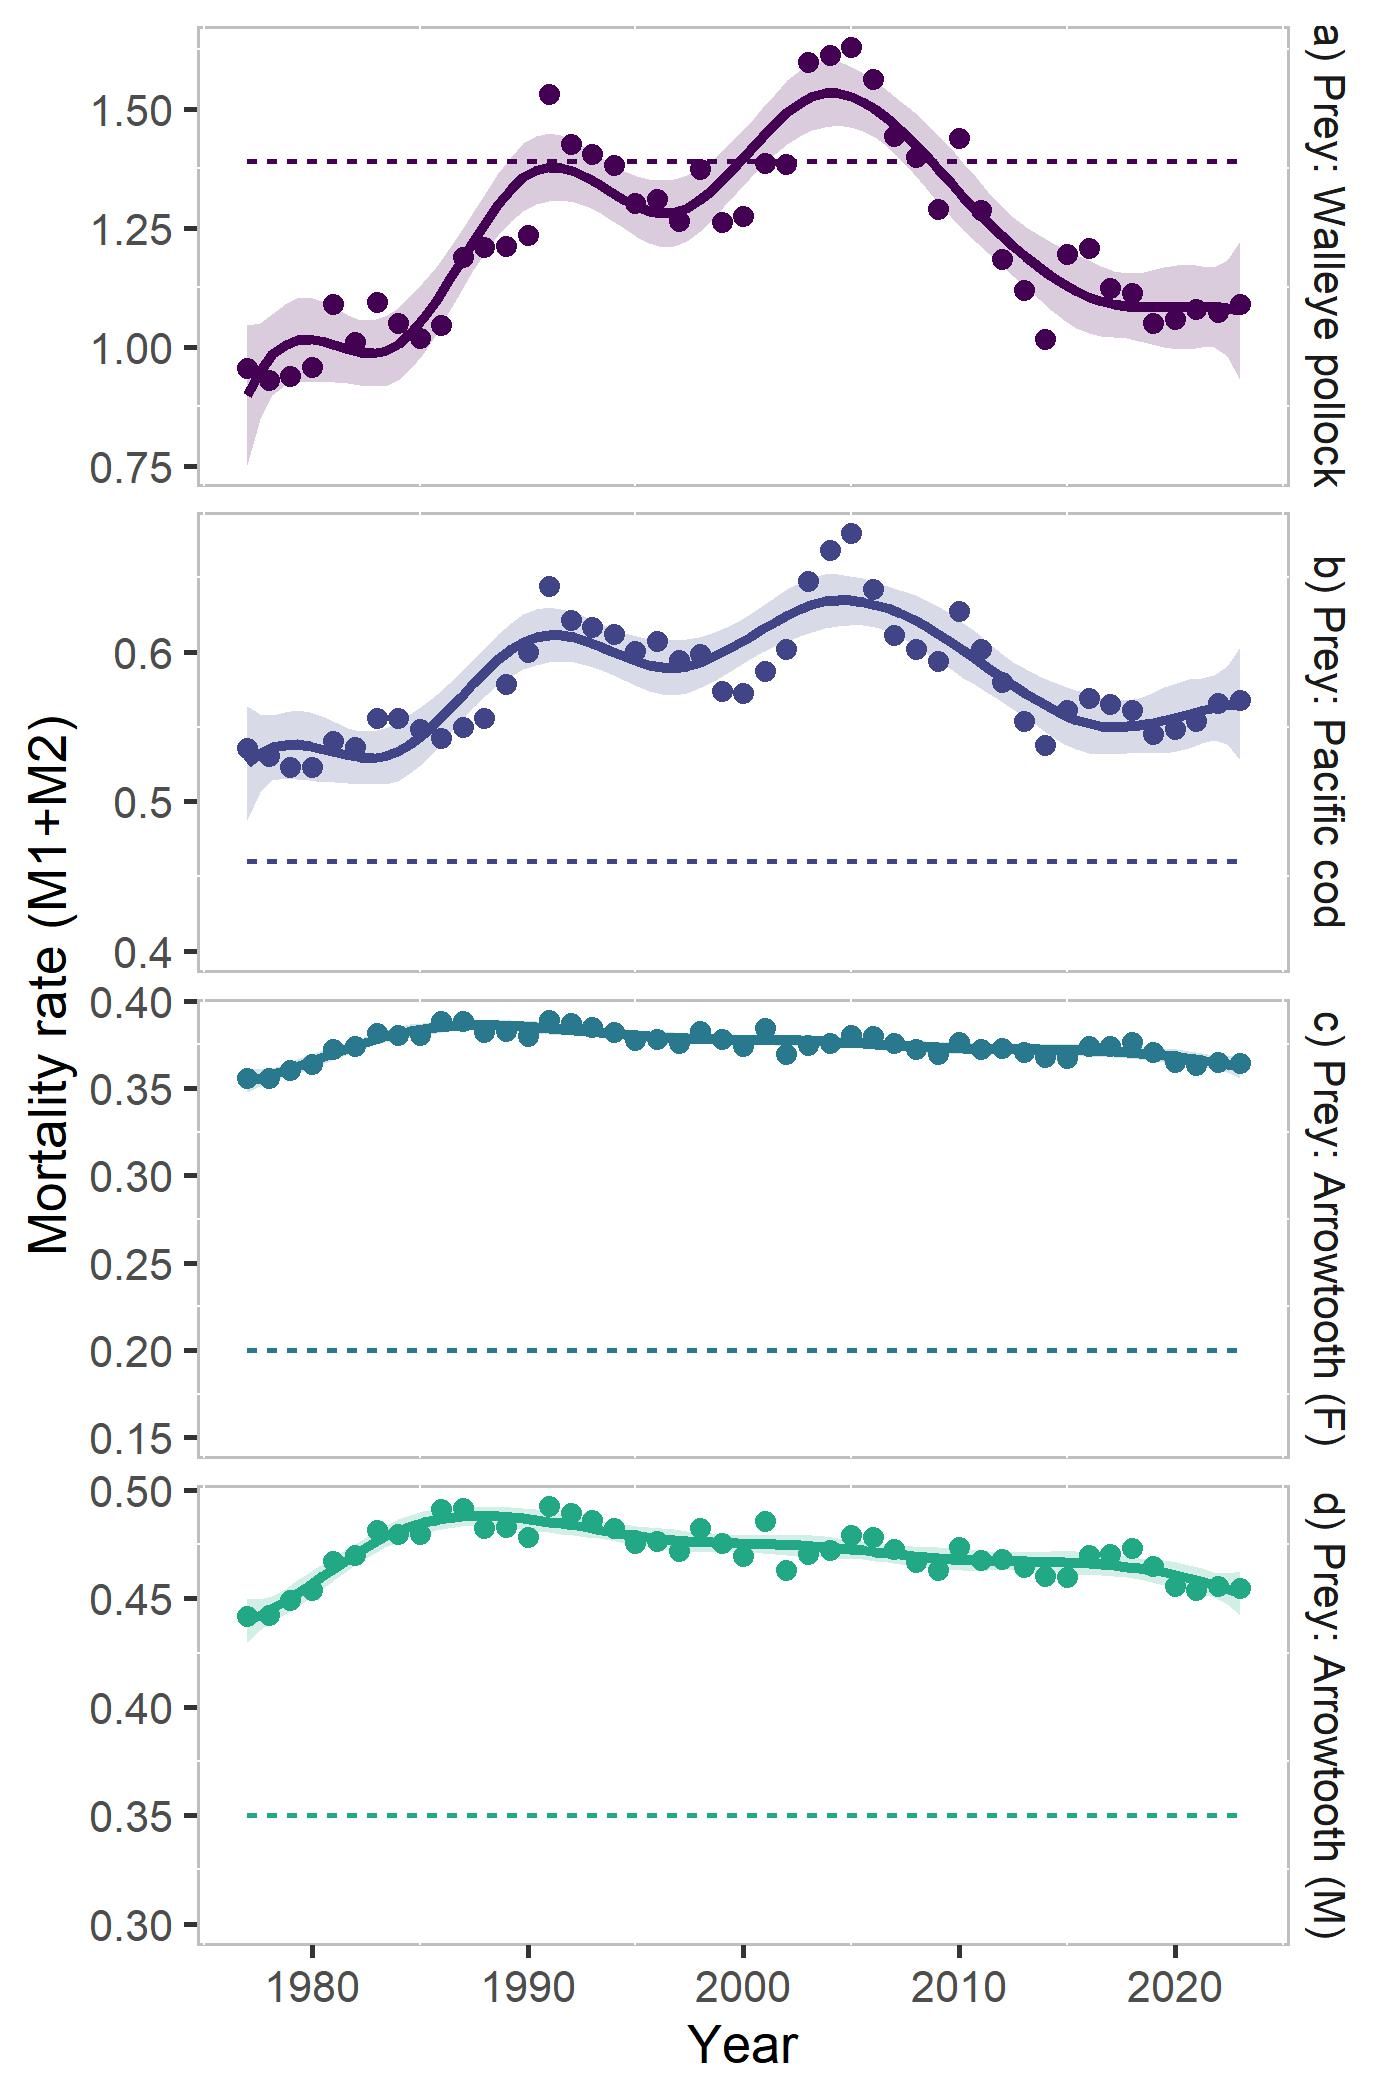
\includegraphics{Results/ESR_Fig1.jpg}
\caption{Annual variation in natural mortality (\textbf{M1+M2}) of age-1
pollock (a), Pacific cod (b), and arrowtooth flounder (females and
males) (c/d) from the single-species models (dashed line), and the
multi-species models with temperature (points; solid line is a loess
polynomial smoother indicating trends over time)}
\end{figure}

\begin{figure}
\centering
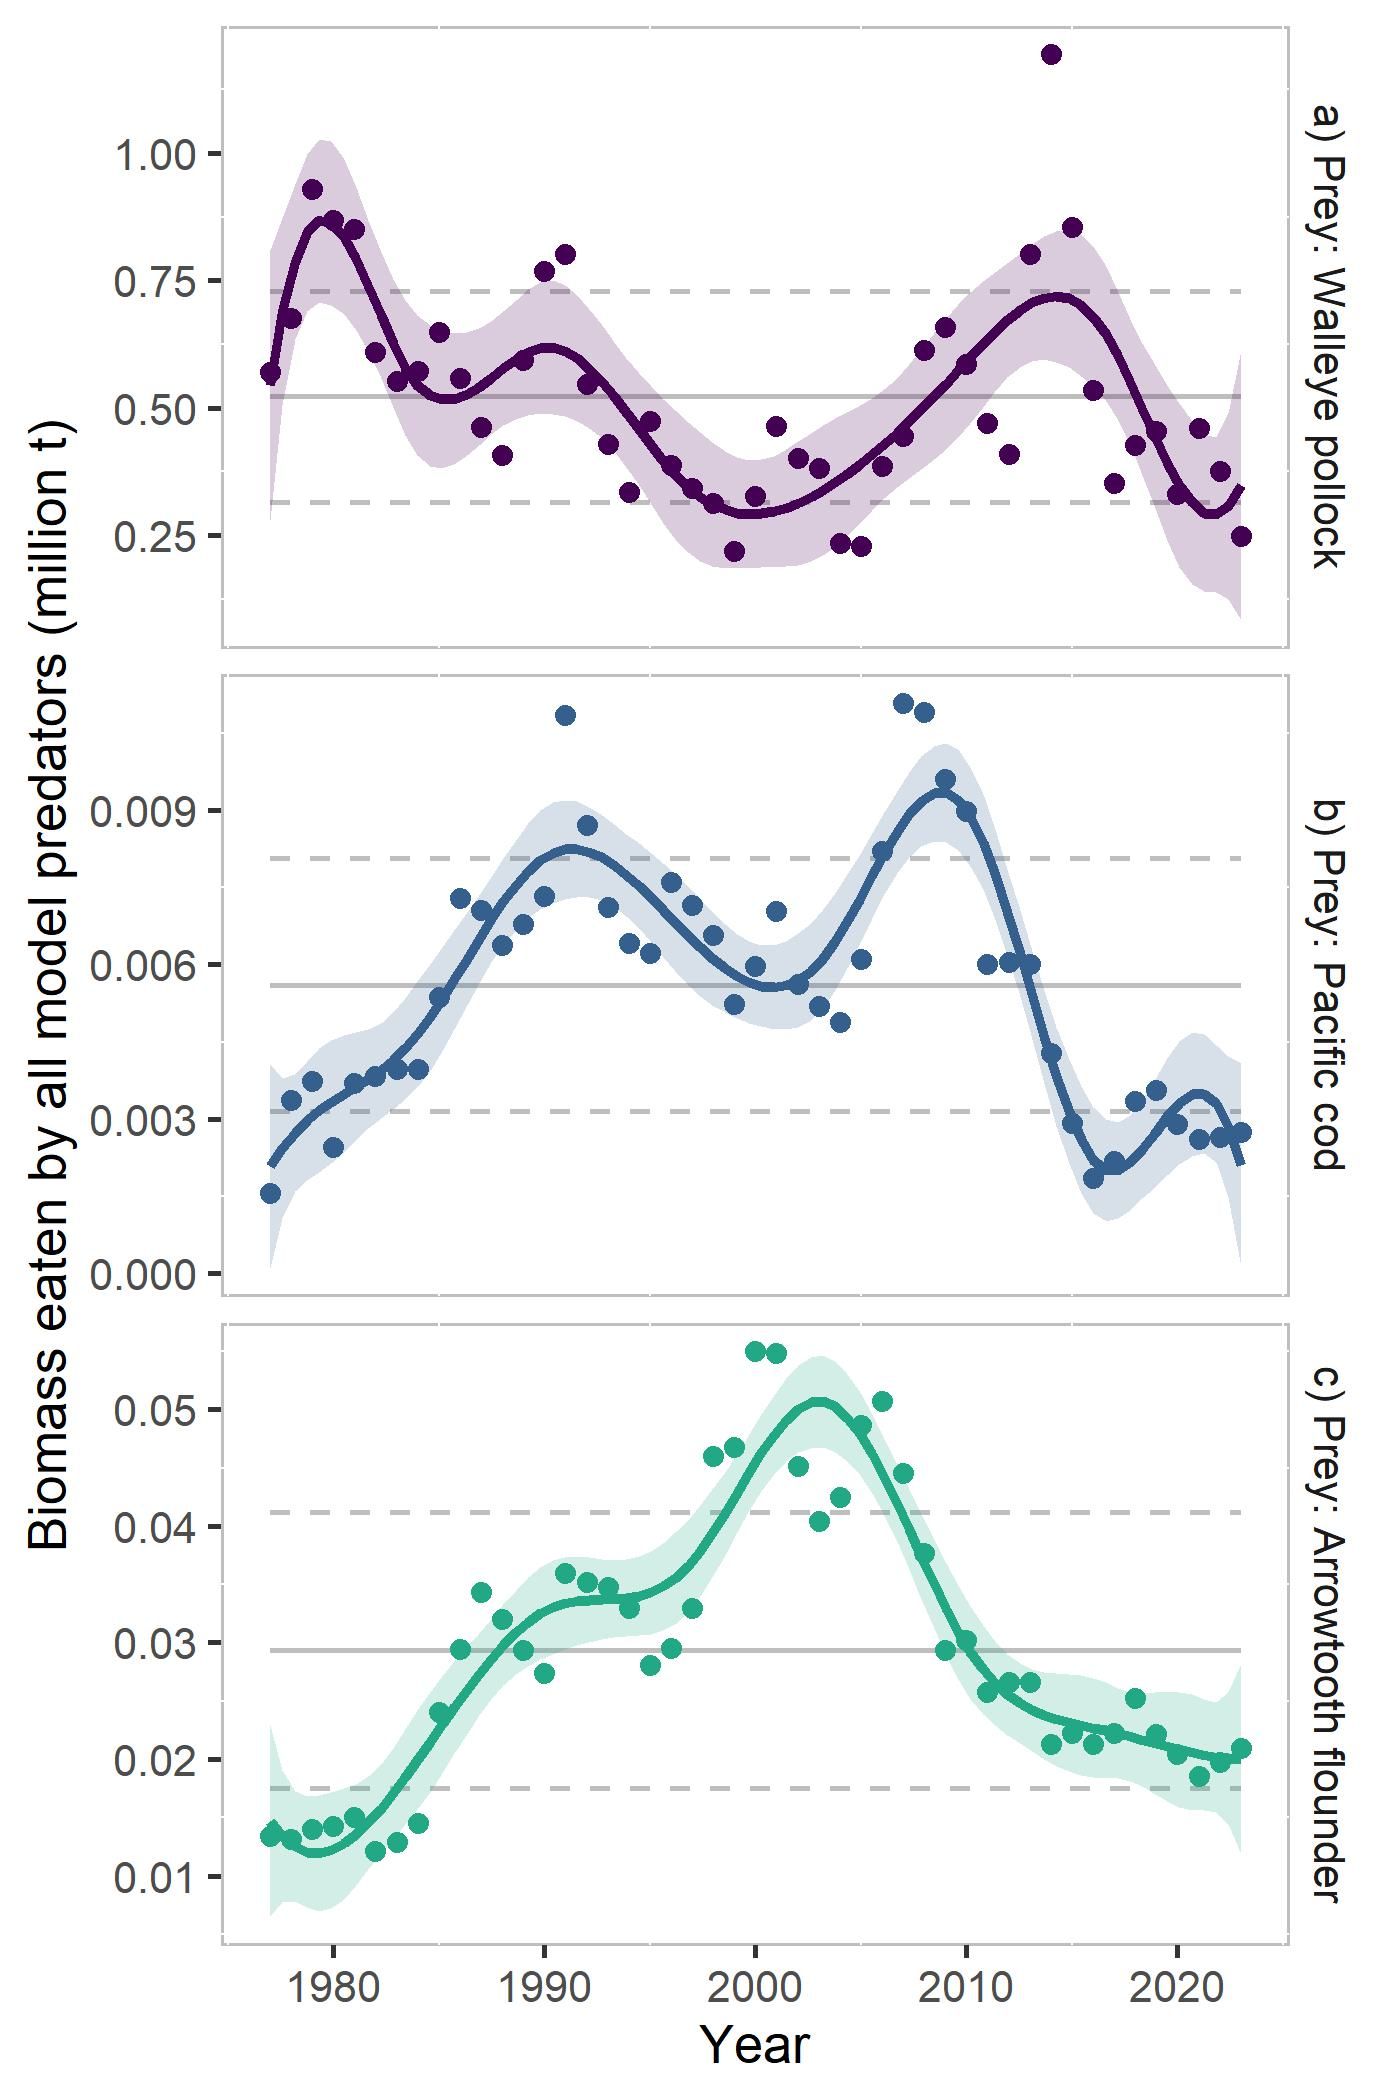
\includegraphics{Results/ESR_Fig2.jpg}
\caption{Multispecies estimates of biomass consumed as prey across all
ages by all predators annually in the model of walleye pollock (a),
Pacific cod (b), and arrowtooth flounder (c). Points represent annual
estimates, gray lines indicate 1979-2023 mean estimates for each
species, and the solid line is a 10 year (symmetric) loess polynomial
smoother indicating trends over time.}
\end{figure}

\begin{figure}
\centering
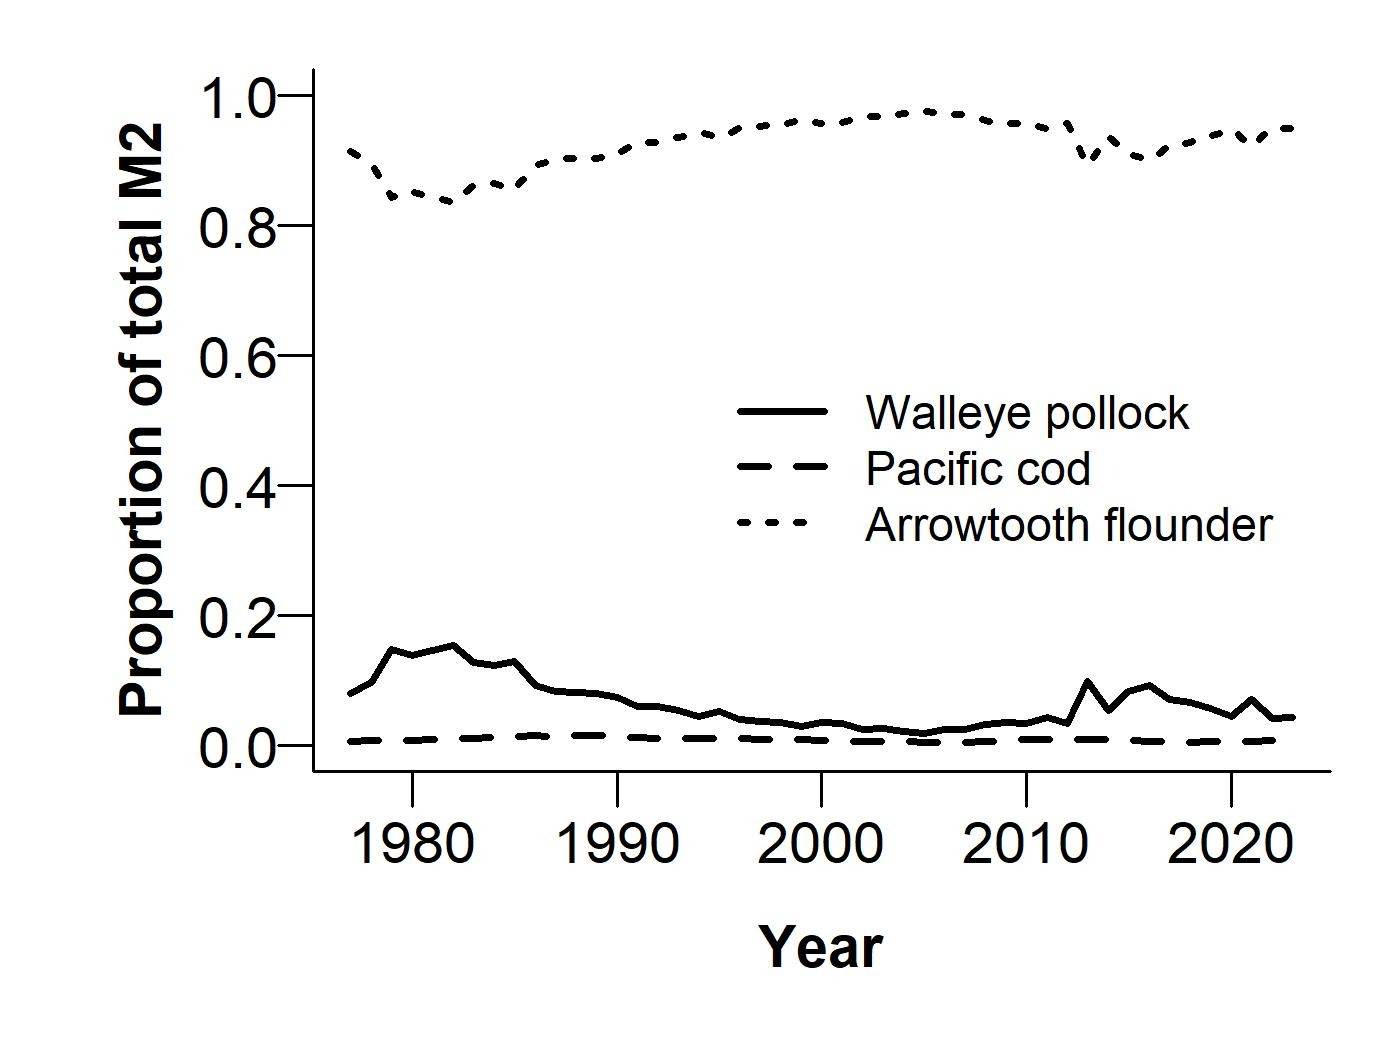
\includegraphics{Results/ESR_Fig3.jpg}
\caption{Proportion of total predation mortality for age-1 pollock from
pollock (solid), Pacific cod (dashed), and arrowtooth flounder (dotted)
predators across years. Updated from Adams et al.~2022.}
\end{figure}

\begin{figure}
\centering
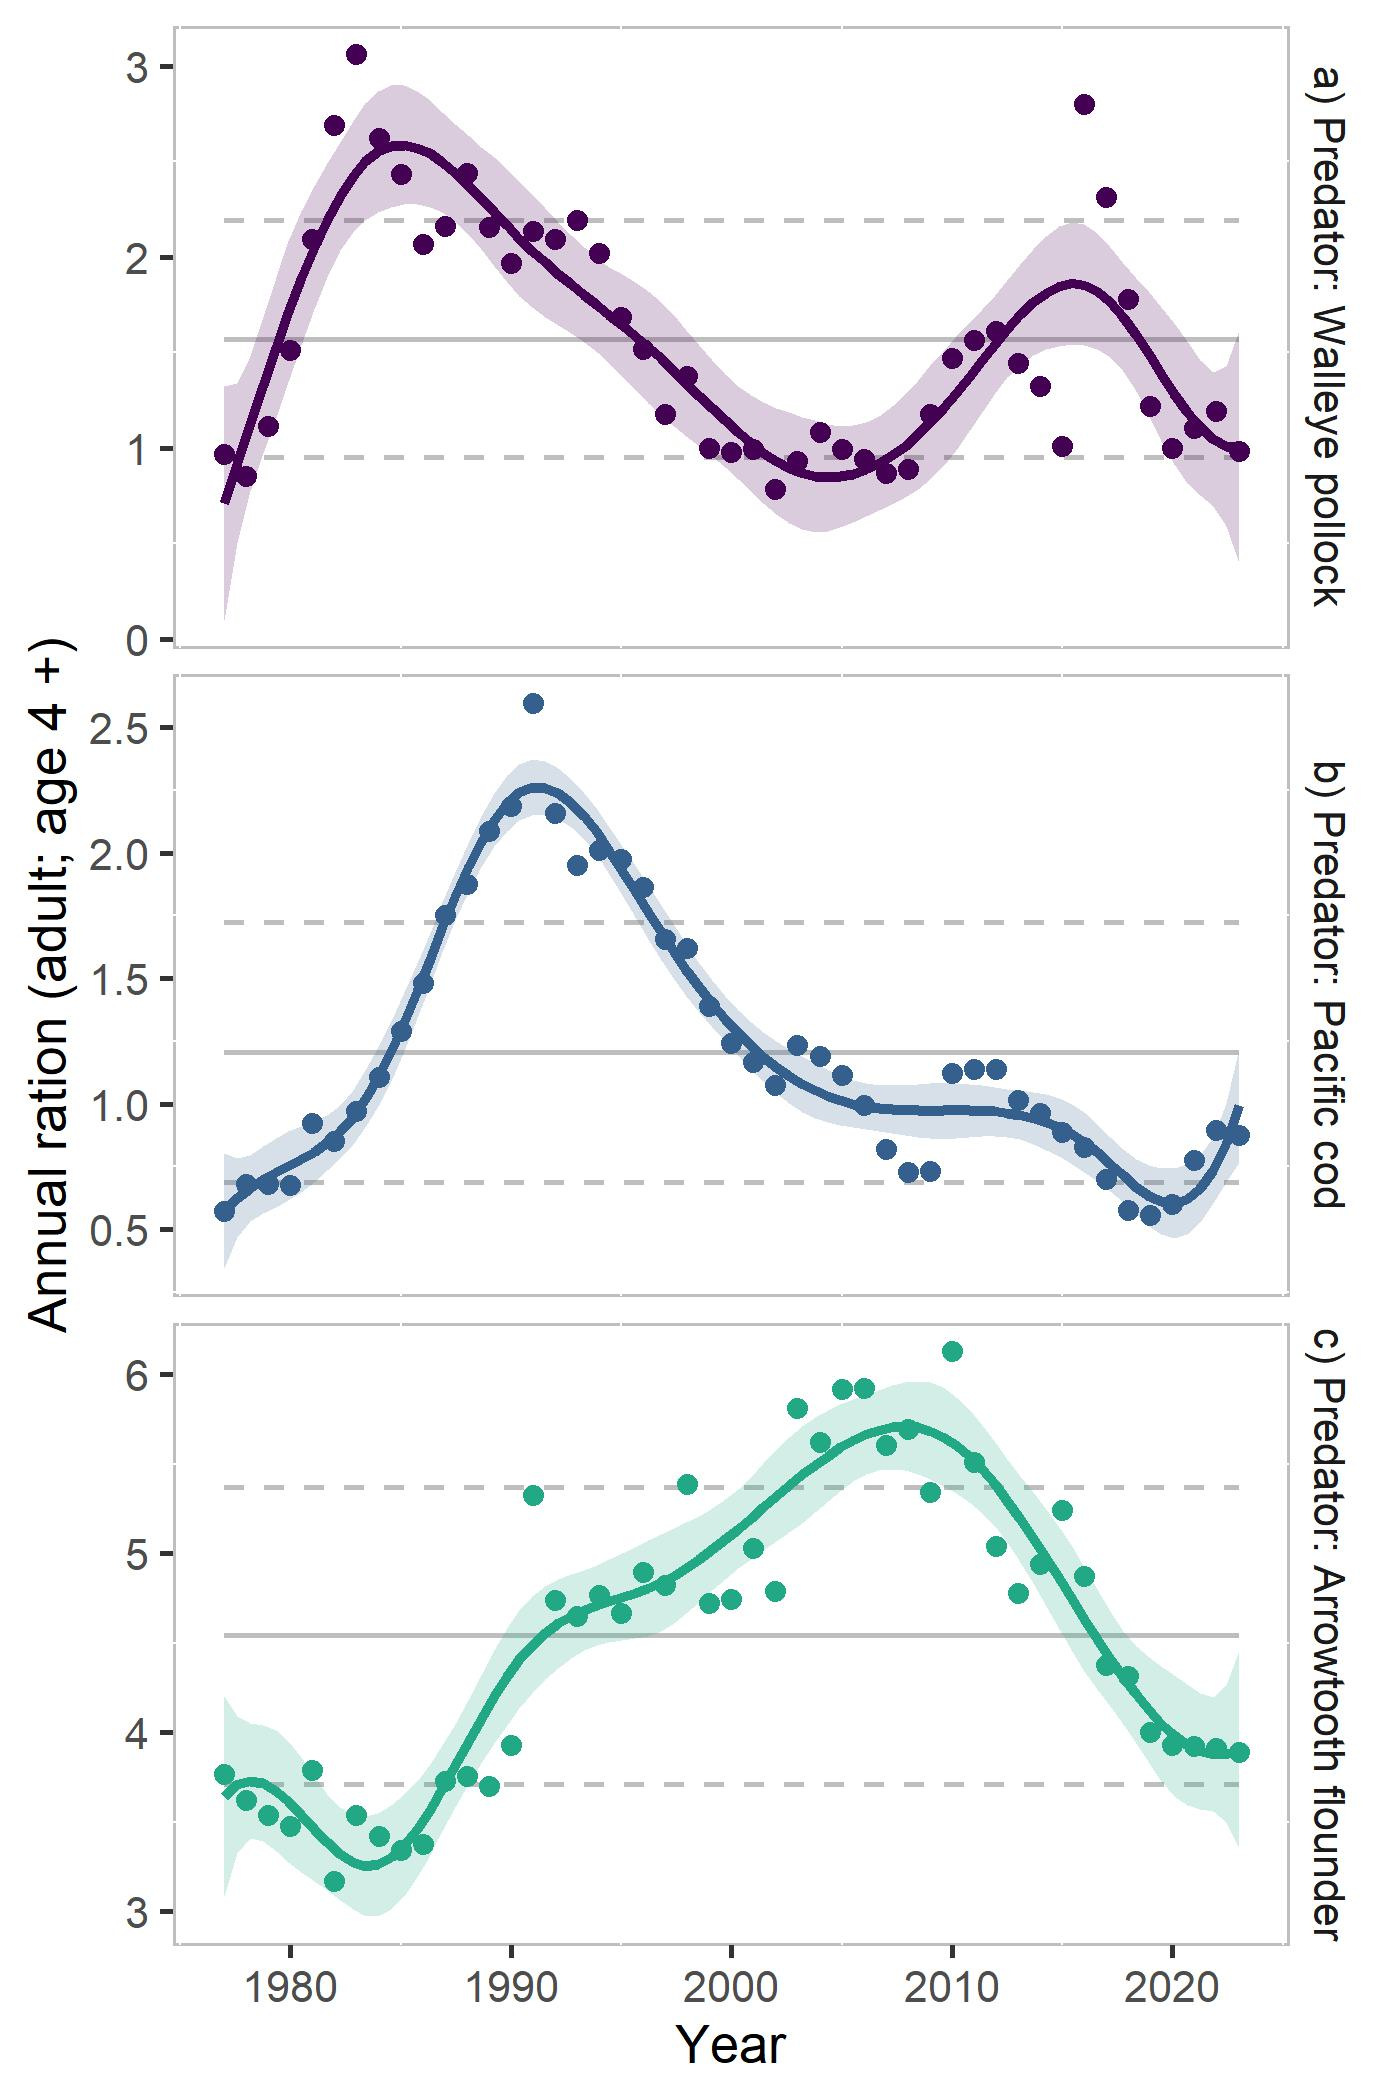
\includegraphics{Results/ESR_Fig4.jpg}
\caption{Multispecies estimates of annual ration (hundred thousand tons
consumed per species per year) for adult (age 4 +) predators: pollock
(a), Pacific cod (b), and arrowtooth flounder (c). Gray lines indicate
1979 -2023 mean estimates and 1 SD for each species; solid line is a 10
y (symmetric) loess polynomial smoother indicating trends in ration over
time.}
\end{figure}

\end{document}
